%==============================================================================
% SIMTiX: A Compact Open-Source SIMT Accelerator for RISC-V
% IEEE conference-format manuscript (IEEEtran).
% Build:  pdflatex simtix && pdflatex simtix   (run twice for cross-references)
% Figures are produced by docs/plot_bench.py into docs/figs/.
%==============================================================================
\documentclass[conference]{IEEEtran}
\IEEEoverridecommandlockouts

\usepackage{cite}
\usepackage{amsmath,amssymb}
\usepackage{graphicx}
\usepackage{booktabs}
\usepackage{listings}
\usepackage{xcolor}
\usepackage{url}
\usepackage[hidelinks]{hyperref}

\graphicspath{{../figs/}}

\lstset{
  basicstyle=\ttfamily\scriptsize,
  columns=fullflexible,
  keepspaces=true,
  breaklines=true,
  frame=single,
  numbers=none,
  aboveskip=4pt, belowskip=4pt
}

\begin{document}

\title{SIMTiX: A Compact, Fully-Open SIMT Accelerator\\ for RISC-V with an Energy-Aware Divergence Study}

\author{\IEEEauthorblockN{Krishna Gorai}
\IEEEauthorblockA{Indian Institute of Technology Mandi\\
Email: kg05112001@gmail.com}}

\maketitle

\begin{abstract}
Open, readable hardware for studying Single-Instruction Multiple-Thread (SIMT)
execution remains scarce: existing open GPGPU cores are large and difficult to
bring up, while teaching cores rarely reach a real implementation flow. We
present \textbf{SIMTiX}, a compact open-source SIMT accelerator attached to a
five-stage RISC-V host through a memory-mapped offload interface. SIMTiX
implements the full SIMT toolbox in a small, synthesizable design: eight lanes
organized into hardware warps, a round-robin scheduler with a background memory
engine for latency hiding, address coalescing on a cache-line-wide data port, a
per-warp SIMT reconvergence stack for control divergence, and an on-chip
scratchpad for data reuse. A key implementation result is that placing the
vector register file and scratchpad in distributed RAM (LUTRAM) shrinks the
design from 74\% to 13\% of the LUTs of a Xilinx Zynq UltraScale+ device while
closing timing at 100~MHz. We characterize SIMTiX with a six-kernel benchmark
suite spanning streaming, stencil, reduction, and data-dependent control-flow
workloads, verified bit-exact against a golden model at sizes up to 1024
threads. Against the scalar host CPU executing the same work, SIMTiX achieves
$7$--$10\times$ speedup on streaming kernels, $2.8\times$ on a
divergence-heavy kernel, and---reported honestly---a slowdown on a serial
reduction, exposing where the SIMT model does and does not pay off. Using the
SIMT active mask as a per-lane clock-enable, we quantify the lane-datapath
dynamic energy a divergence-aware gated design saves (up to 22.5\% on a
divergent kernel). We further extend each lane with a single-cycle
floating-point unit supporting both single and half precision (FP32 and FP16):
half precision reuses the single-precision datapath through NaN-boxed
widen--compute--narrow, which we show is correctly single-rounded and adds no
extra cycles. The unit is verified bit-exact against an IEEE-754 reference over
$76{,}048$ vectors, and sustains the engine's full lane-parallel throughput. The
complete RTL, benchmark harness, and FPGA flow are publicly available.
\end{abstract}

\begin{IEEEkeywords}
SIMT, GPGPU, RISC-V, hardware accelerator, control divergence, memory
coalescing, floating-point, half precision, FPGA, clock gating, open-source
hardware.
\end{IEEEkeywords}

%==============================================================================
\section{Introduction}
%==============================================================================
Graphics processing units execute thousands of scalar threads in lockstep groups
called \emph{warps} under a Single-Instruction Multiple-Thread (SIMT) model. The
microarchitectural mechanisms that make this efficient---warp scheduling for
latency hiding, memory coalescing, control-divergence handling, and on-chip
scratchpads---are well documented at the level of commercial GPUs, but they are
hard to \emph{study in RTL}. Production GPUs are proprietary; open GPGPU cores
such as Vortex~\cite{vortex} are powerful but large and complex to bring up; and
the small academic cores are often simulator-only or stop short of a real
implementation flow.

This paper presents \textbf{SIMTiX}, a deliberately compact open-source SIMT
accelerator for RISC-V whose entire path---RTL, simulation, synthesis,
place-and-route, bitstream, and post-route gate-level sign-off---is reproducible
on a single workstation with free or widely available tools. SIMTiX is small
enough to read end-to-end yet implements the complete SIMT mechanism set, and we
use it to produce a measured, honest evaluation rather than a demonstration.

\noindent\textbf{Contributions.}
\begin{itemize}
\item A compact, fully-open SIMT accelerator (eight lanes, four resident warps)
integrated with a five-stage RISC-V host as a self-contained
system-on-chip, exercising the entire RTL-to-bitstream flow
(Sections~\ref{sec:arch}--\ref{sec:impl}).
\item An implementation study showing that moving the vector register file and
scratchpad into distributed RAM reduces LUT usage by $5.7\times$ and closes
100~MHz timing, with a clear analysis of why the register-file read multiplexer,
not the ALUs, dominates a naive SIMT datapath (Section~\ref{sec:impl}).
\item A six-kernel benchmark suite, verified bit-exact at up to 1024 threads,
that isolates distinct microarchitectural behaviors, and a \emph{measured}
speedup against the scalar host---including a deliberately reported case where
SIMT loses (Section~\ref{sec:results}).
\item A divergence-aware lane clock-gating energy model that reuses the SIMT
active mask as a per-lane clock-enable and quantifies the lane-datapath energy
saved as a function of control divergence (Sections~\ref{sec:arch},
\ref{sec:results}).
\item A per-lane floating-point extension covering both FP32 and FP16, in which
half precision is obtained almost for free from the single-precision path via
NaN-boxed widen--compute--narrow (which we show is correctly single-rounded),
verified bit-exact and shown to sustain the engine's full lane-parallel
throughput (Section~\ref{sec:fp}).
\end{itemize}

%==============================================================================
\section{Background: the SIMT execution model}
%==============================================================================
A SIMT machine groups scalar \emph{threads} into \emph{warps} that share one
instruction stream and execute on a vector of \emph{lanes}. SIMTiX uses a warp
size equal to its lane count ($\mathrm{WARP\_SIZE}=\mathrm{NUM\_LANES}=8$), so
one warp occupies all lanes for one instruction. Multiple warps are resident
simultaneously ($\mathrm{NUM\_WARPS}=4$) and time-share a single
fetch/decode/execute datapath; when one warp stalls on memory, the scheduler
issues another, hiding latency. Three effects determine SIMT efficiency:
\emph{occupancy} (enough warps to hide latency), \emph{memory coalescing}
(merging lanes' accesses into wide transactions), and \emph{control divergence}
(lanes within a warp taking different branch outcomes, which serializes the
divergent paths). SIMTiX implements hardware for all three and instruments each
so they can be measured.

%==============================================================================
\section{SIMTiX Architecture}\label{sec:arch}
%==============================================================================
SIMTiX is an offload accelerator. The host RISC-V core programs a command block
over a memory-mapped (MMIO) register interface---kernel entry PC, base pointers
\texttt{A/B/C}, and thread count \texttt{N}---then writes a \texttt{GO} bit and
polls a \texttt{DONE} status bit. On \texttt{GO} the accelerator launches a grid
of \texttt{N} threads as $\lceil N/8\rceil$ warps. Each thread receives its
identity and arguments through a register-seeding convention at spawn
(\texttt{a0}=thread id, \texttt{a1..a3}=base pointers, \texttt{a4}=\texttt{N}).

\subsection{Warp pool, scheduler, and latency hiding}
The warp pool holds four resident warp slots, each with its own architectural
state (program counter, active mask, register file partition, and reconvergence
stack), all sharing one datapath and one data port. A round-robin scheduler
issues one runnable warp per cycle. Memory instructions are handed to a
\emph{background memory engine} that services the access while the scheduler
keeps issuing \emph{other} warps' compute instructions on the otherwise-idle
datapath---the classic GPU latency-hiding trick. At most one memory instruction
is in flight (single data port); a warp that wants memory while the port is busy
simply waits its turn without blocking others.

\subsection{Per-lane datapath and the register file}
Each lane is a single-cycle RV32IM integer datapath (add/sub, logic, shifts,
set-less-than, and \texttt{mul}; no divide or floating point). The vector
register file (VRF) is logically $\mathrm{NUM\_WARPS}\times\mathrm{NUM\_LANES}
\times 32$ words. A naive flip-flop VRF is the dominant cost of the design
(Section~\ref{sec:impl}); SIMTiX instead implements it as one distributed-RAM
bank per lane, addressed by \{warp, register\}, with one synchronous write port
and two asynchronous read ports.

\subsection{Memory coalescing}
The data port is one cache line wide ($\mathrm{LINE\_WORDS}=8$, 256~bits). When a
warp issues a load or store, the memory engine groups the active lanes' effective
addresses by line and spends one transaction per distinct line. A contiguous
warp access (e.g.\ \texttt{A[tid]}) collapses to a single line transaction, while
a fully scattered access costs up to eight. A debug counter records line
transactions, making coalescing efficiency directly measurable.

\subsection{Control divergence: the reconvergence stack}\label{sec:diverge}
Each warp owns a small SIMT reconvergence stack. The top-of-stack frame defines
the warp's live PC and \emph{active mask} (which lanes execute). A branch is
resolved per lane: if all active lanes agree, the PC is simply retargeted; if
they disagree, a frame is pushed so the two lane groups run in turn and
reconverge at a join PC. SIMTiX supports the compiler-free convention of
single-sided \texttt{if} and divergent loops: a forward branch reconverges at its
target, a backward branch at the fall-through. A divergence counter records each
divergent branch event.

\subsection{On-chip scratchpad}
A per-warp scratchpad (64 words/warp) occupies a dedicated address aperture.
Accesses that fall in the aperture are serviced from on-chip RAM and never reach
the global data port, so data reused across a warp's lanes (for example a
broadcast matrix row) can be staged once and reused, cutting global traffic.

\subsection{Divergence-aware lane clock-gating}\label{sec:gating}
The active mask is exactly the set of lanes doing useful work; masked-off lanes
produce no architectural change yet, in a baseline design, still clock their
pipeline registers. SIMTiX treats the active mask as a per-lane clock-enable: the
mask drives an integrated clock-gate on each lane's registers, so only active
lanes are clocked. Let an issued instruction activate $a$ of $L$ lanes. An
ungated design clocks $L$ lanes; a gated design clocks $a$. Summing over a
kernel, the lane-datapath dynamic energy a gated design saves is
\begin{equation}
E_{\text{saved}} = 1 - \frac{\sum_i a_i}{L \cdot \sum_i 1}
                 = 1 - \frac{\text{active-lane instructions}}{L \cdot \text{issued instructions}} .
\label{eq:energy}
\end{equation}
Two hardware counters---issued instructions and summed active lanes---make
Eq.~\eqref{eq:energy} directly observable.

%==============================================================================
\section{Implementation}\label{sec:impl}
%==============================================================================
SIMTiX is written in synthesizable SystemVerilog and integrated with a reused
five-stage RV32I host pipeline into a self-contained chip
(\texttt{chip\_top}): host core, driver ROM, accelerator, and an eight-bank
on-chip shared memory. In the integrated chip the host loads the operands into
shared memory, launches the accelerator, reads the results back, and publishes a
checksum---the whole CPU$\rightarrow$memory$\rightarrow$accelerator$\rightarrow$
memory$\rightarrow$CPU loop runs in hardware.

\subsection{From flip-flops to LUTRAM}
The first synthesis of the accelerator on a Zynq UltraScale+
(\texttt{xczu7ev}) consumed 170{,}868 LUTs---74\% of the device---at only 10\%
of its flip-flops, and topped out near 122~MHz. The cause is structural: a
flip-flop VRF of $4\times8\times32$ 32-bit words is 32{,}768 registers read as
\texttt{vrf[warp][lane][reg]} with \emph{both} warp and register variable, i.e.\
a 128-to-1 multiplexer per lane per read port. That multiplexer fabric, not the
ALUs, dominates area and sets the critical path. Re-expressing the VRF as one
distributed-RAM bank per lane, and likewise moving the scratchpad into LUTRAM,
removes essentially all of those registers. Table~\ref{tab:ppa} summarizes the
effect: LUTs fall by $5.7\times$ and the design closes 100~MHz timing with
positive slack.

\begin{table}[t]
\caption{Accelerator PPA on Xilinx \texttt{xczu7ev} before/after moving the VRF
and scratchpad to distributed RAM (out-of-context synthesis).}
\label{tab:ppa}
\centering
\footnotesize
\begin{tabular}{lrrr}
\toprule
 & FF-based VRF & \multicolumn{2}{c}{LUTRAM VRF+scratch}\\
\cmidrule(lr){2-2}\cmidrule(lr){3-4}
Metric & baseline & after & $\Delta$\\
\midrule
LUTs            & 170{,}868 (74\%) & 30{,}088 (13\%) & $-82\%$\\
Flip-flops      & 44{,}112 (10\%)  & 4{,}590 (1.0\%) & $-90\%$\\
DSP48E2         & 24               & 24             & --\\
BRAM            & 0                & 0              & --\\
Timing (100~MHz)& WNS $-3.21$~ns   & WNS $+2.25$~ns & met\\
Power           & 1.67~W @200~MHz  & 0.81~W @100~MHz& --\\
\bottomrule
\end{tabular}
\end{table}

\subsection{Full-chip place-and-route}
The complete chip was taken through opt/place/phys-opt/route to a bitstream on
\texttt{xczu7ev}. Post-route it meets all timing at 100~MHz (setup
WNS $+0.000$~ns, hold met) and uses 34{,}850 LUTs (15.1\%), 6{,}130 flip-flops
(1.3\%), 3{,}348 LUTRAM, 24 DSP, and zero BRAM, at 1.09~W. The accelerator is
$\sim$87\% of the logic; the host core and 4~KB shared memory are small by
comparison.

\subsection{Verification ladder}
Correctness is established at four levels: (i) cycle-accurate RTL simulation with
self-checking testbenches (Verilator); (ii) behavioral simulation in the vendor
GUI; (iii) full place-and-route with post-route timing sign-off; and (iv)
post-implementation \emph{gate-level} functional simulation of the routed netlist
(UNISIM primitives), which reproduces the integrated chip's golden checksum of
964 bit-for-bit. The benchmark suite below adds a fifth, breadth-oriented level.

%==============================================================================
\section{Methodology}\label{sec:method}
%==============================================================================
\subsection{Benchmark suite}
We wrote six kernels, each chosen to stress a distinct mechanism
(Table~\ref{tab:kernels}). All are assembled from RISC-V source with a stock
toolchain. Each runs at $N\in\{8,64,256,1024\}$ threads (the divergence-heavy
\texttt{collatz} to 256), and every output element is checked against a golden
model computed in the testbench.

\begin{table}[t]
\caption{Benchmark kernels and the mechanism each one stresses.}
\label{tab:kernels}
\centering
\footnotesize
\begin{tabular}{lll}
\toprule
Kernel & Computation & Stresses\\
\midrule
\texttt{vadd}    & $C_i=A_i+B_i$                  & baseline streaming\\
\texttt{saxpy}   & $C_i=3A_i+B_i$                 & coalescing, \texttt{mul}\\
\texttt{fir}     & $C_i=A_i+2A_{i+1}+A_{i+2}$     & stencil, partial coalescing\\
\texttt{relu}    & $C_i=\max(0,A_i)$              & data-dependent light divergence\\
\texttt{collatz} & Collatz step count            & data-dependent heavy divergence\\
\texttt{reduce}  & $C_w=\sum_{l=0}^{7}A_{8w+l}$   & scratchpad + reduction\\
\bottomrule
\end{tabular}
\end{table}

\subsection{Metrics}
Per run the engine reports cycles (launch to done), global line transactions,
scratchpad transactions, divergent-branch events, issued instructions, and
summed active lanes. From these we derive lane utilization
$\sum a_i/(L\sum 1)$ and a scalar-equivalent throughput
$\sum a_i/\text{cycles}$ (work retired per cycle).

\subsection{Measured scalar baseline}
For an apples-to-apples speedup, each kernel is also implemented as a natural
scalar loop and executed on the \emph{same} five-stage host pipeline in RTL,
counting cycles from program start to completion. The host is pure RV32I, so
constant multiplies are lowered to shift-and-add; \texttt{matmul}, which needs a
general multiply, is therefore excluded from the scalar comparison. The scalar
program and the accelerator are checked to produce identical results.

%==============================================================================
\section{Results}\label{sec:results}
%==============================================================================
\subsection{Throughput and latency hiding}
Figure~\ref{fig:throughput} plots scalar-equivalent throughput against problem
size. With only eight threads (one warp) throughput is low---there is nothing to
hide memory latency behind---but it climbs as more warps become resident and
saturates near 6.5--6.7 work-items/cycle for the coalesced kernels, out of an
ideal of 8. The gap is the single data port: while one warp's coalesced access
occupies the memory engine, only three other warps are available to fill the
datapath.

\begin{figure}[t]
\centering
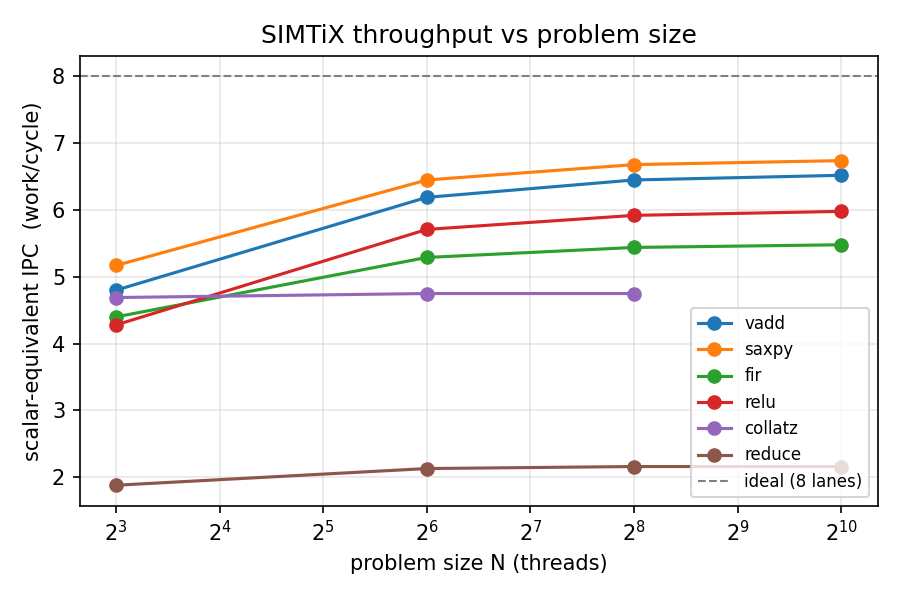
\includegraphics[width=\columnwidth]{throughput.png}
\caption{Scalar-equivalent throughput versus problem size. Throughput ramps as
occupancy rises (latency hiding) and saturates below the 8-lane ideal due to the
single shared data port.}
\label{fig:throughput}
\end{figure}

\subsection{Memory coalescing}
Figure~\ref{fig:mem} shows global line transactions versus size.
\texttt{saxpy}/\texttt{vadd} are perfectly coalesced (three line transactions per
warp---one each for \texttt{A}, \texttt{B}, \texttt{C}), whereas the
\texttt{fir} stencil reads \texttt{A[i]}, \texttt{A[i+1]}, \texttt{A[i+2]}; the
shifted reads straddle line boundaries and double its traffic. This is the
expected signature of \emph{partial} coalescing and explains \texttt{fir}'s lower
speedup. A deliberately scattered access (stride 8) costs the full eight
transactions per warp---an $8\times$ traffic increase that coalescing removes for
contiguous data.

\begin{figure}[t]
\centering
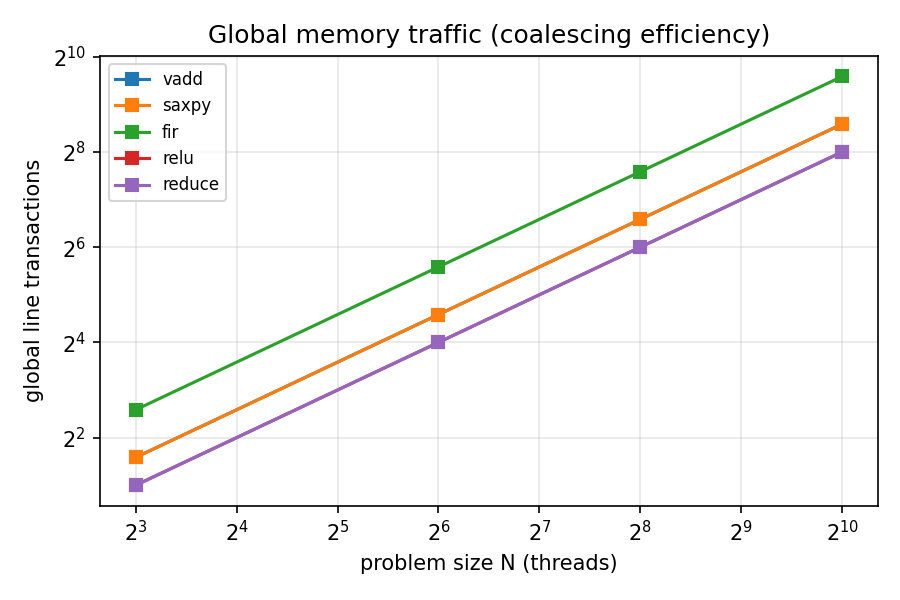
\includegraphics[width=\columnwidth]{memtraffic.png}
\caption{Global line transactions versus size. Contiguous kernels coalesce to
three transactions per warp; the \texttt{fir} stencil's shifted reads straddle
lines and roughly double the traffic.}
\label{fig:mem}
\end{figure}

\subsection{Control divergence and lane utilization}
Figure~\ref{fig:util} reports lane utilization. The convergent streaming kernels
keep all eight lanes active every instruction (100\%). \texttt{relu} diverges
only where the input changes sign, dropping utilization slightly to 93.7\%.
\texttt{collatz}, whose per-lane trip count is data-dependent, falls to 68.3\% as
finished lanes mask off while others continue. \texttt{reduce} is lowest (39.8\%)
because its second phase collapses eight lanes' partial sums on a single lane.
Per Eq.~\eqref{eq:energy}, the unused fraction is the lane-datapath dynamic
energy a clock-gated design saves: from 0\% on convergent code up to 22.5\% on a
divergence-heavy microbenchmark.

\begin{figure}[t]
\centering
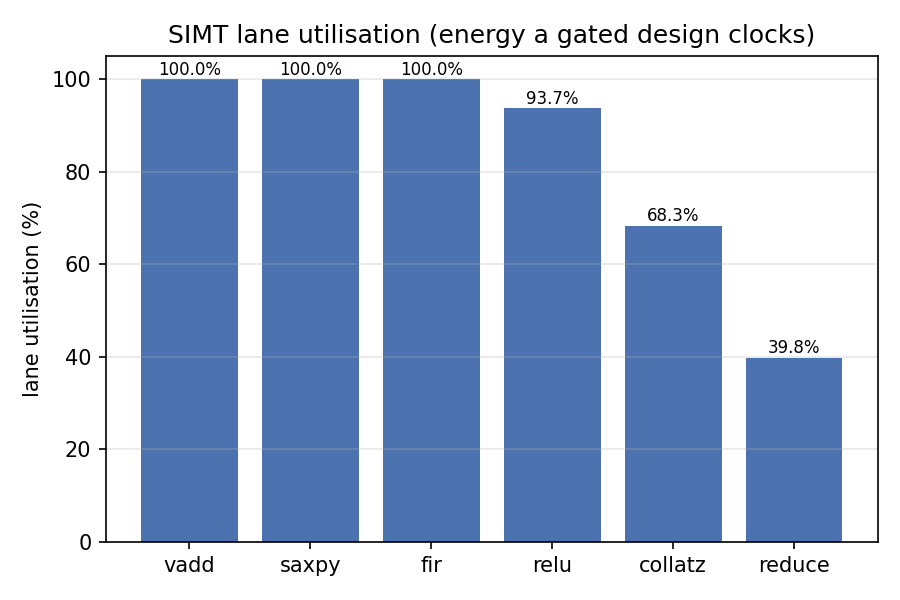
\includegraphics[width=\columnwidth]{laneutil.png}
\caption{SIMT lane utilization per kernel (largest size). The complement is the
lane-datapath dynamic energy a divergence-aware clock-gated design saves
(Eq.~\eqref{eq:energy}).}
\label{fig:util}
\end{figure}

\subsection{Scratchpad data reuse}
For an $8\times8$ matrix-row product, staging the broadcast input row in the
scratchpad once and reusing it cuts global line transactions from 17 to 10
(Figure~\ref{fig:locality}). At this small size the staged version spends more
cycles (the scratchpad is single-ported and serializes the stage-in), so the win
is in off-chip traffic rather than latency---an honest trade that grows with data
size and reuse distance.

\begin{figure}[t]
\centering
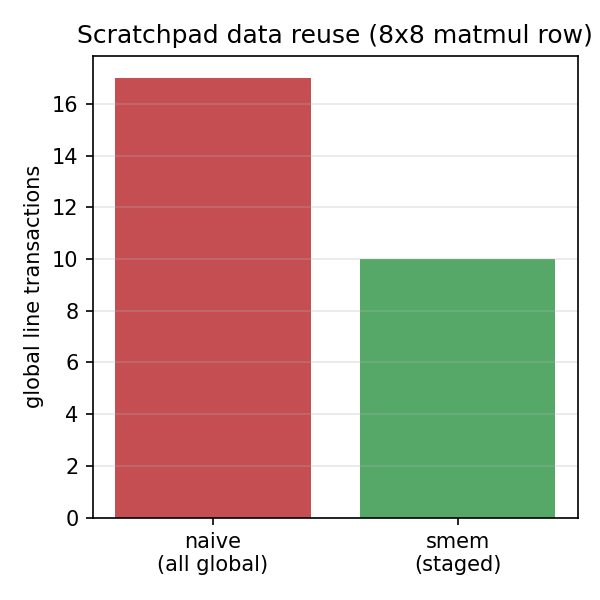
\includegraphics[width=0.72\columnwidth]{locality.png}
\caption{Global line transactions for an $8\times8$ matmul row: staging the
reused row in the scratchpad cuts off-chip traffic.}
\label{fig:locality}
\end{figure}

\subsection{Measured speedup over the scalar host}
Figure~\ref{fig:speedup} and Table~\ref{tab:speedup} give the headline result:
measured accelerator speedup over the scalar host executing identical work.
Streaming kernels reach $7$--$10\times$, approaching the eight-lane width scaled
by the coalescing traffic reduction. \texttt{fir} is lower ($7.0\times$) because
of its partial coalescing. \texttt{collatz} achieves $2.8\times$: heavy
data-dependent divergence erodes---but does not eliminate---the SIMT advantage.
\texttt{reduce} is below unity ($0.72\times$): its single-lane collapse and
single-ported scratchpad make it \emph{slower} than the scalar core. We report
this case deliberately---the SIMT model is not universally beneficial, and a
reduction needs a better hardware primitive (e.g.\ a tree-reduction network) to
win on this engine.

\begin{figure}[t]
\centering
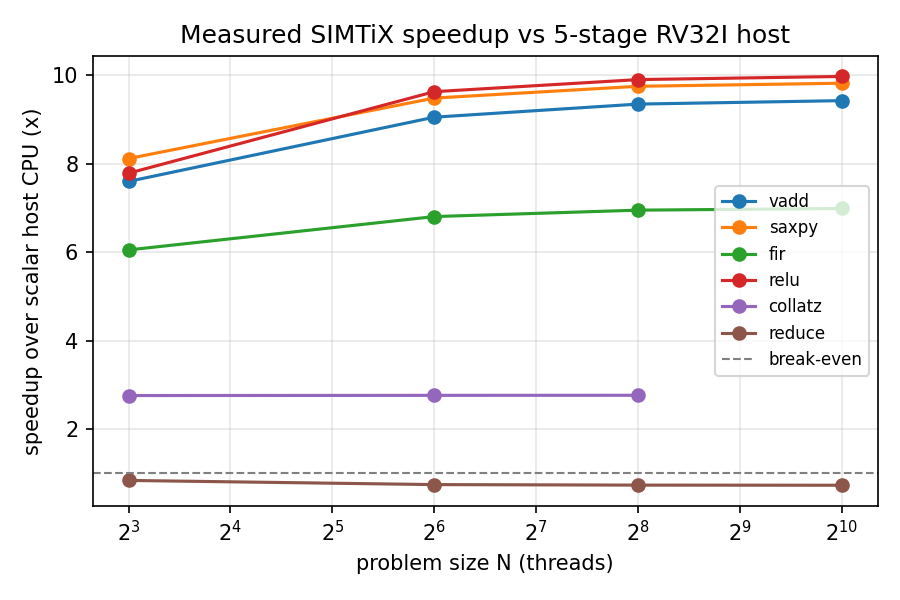
\includegraphics[width=\columnwidth]{speedup.png}
\caption{Measured speedup over the five-stage RV32I host running the same work.
Streaming kernels reach $7$--$10\times$; divergence reduces the gain; the serial
reduction falls below break-even.}
\label{fig:speedup}
\end{figure}

\begin{table}[t]
\caption{Measured cycles and speedup (largest size; \texttt{collatz} at $N{=}256$).
Lane utilization and global traffic from the accelerator counters.}
\label{tab:speedup}
\centering
\footnotesize
\begin{tabular}{lrrrrr}
\toprule
Kernel & $N$ & Accel & CPU & Speedup & Lane-util\\
\midrule
\texttt{vadd}    & 1024 & 1{,}413 & 13{,}322 & $9.43\times$ & 100\%\\
\texttt{saxpy}   & 1024 & 1{,}669 & 16{,}394 & $9.82\times$ & 100\%\\
\texttt{fir}     & 1024 & 2{,}053 & 14{,}345 & $6.99\times$ & 100\%\\
\texttt{relu}    & 1024 & 1{,}284 & 12{,}809 & $9.98\times$ & 93.7\%\\
\texttt{collatz} &  256 & 9{,}637 & 26{,}601 & $2.76\times$ & 68.3\%\\
\texttt{reduce}  & 1024 & 6{,}023 &  4{,}363 & $0.72\times$ & 39.8\%\\
\bottomrule
\end{tabular}
\end{table}

\subsection{Design-space exploration: lanes and warps}\label{sec:dse}
SIMTiX is parameterized in its lane count and resident-warp count
($\mathrm{WARP\_SIZE}=\mathrm{NUM\_LANES}$, and the coalescing line scales with
the lanes). We swept $\mathrm{NUM\_LANES}\in\{4,8,16,32\}$ against
$\mathrm{NUM\_WARPS}\in\{2,4,8\}$---all twelve configurations elaborate and pass
the suite bit-exact---and measured throughput on the five lane-count-agnostic
kernels. Table~\ref{tab:dse} reports the geometric-mean throughput, and
Figure~\ref{fig:dse} plots it against lane count.

Two clear effects emerge. First, throughput scales almost linearly with lanes:
$3.06\rightarrow5.85\rightarrow11.68\rightarrow23.24$ work-items/cycle, about
$1.97\times$ per doubling, i.e.\ $7.6\times$ from 4 to 32 lanes. Widening the
lanes also widens the coalescing line, so global line transactions fall
proportionally (e.g.\ \texttt{vadd} drops $768\rightarrow96$ transactions from 4
to 32 lanes). Second, and more interesting, the resident-warp count makes
essentially no difference here (the three curves in Figure~\ref{fig:dse}
coincide; eight warps is marginally \emph{worse} due to extra spawn bookkeeping).
This is honest about the harness: the behavioral memory model answers in a single
cycle, so there is almost no latency for extra warps to hide; occupancy beyond
the two warps needed to overlap the memory engine with the datapath pays off only
under realistic multi-cycle memory. The two knobs are thus separable---lanes buy
data-parallel throughput, warps buy latency tolerance---and both cost register-file
area ($\propto\!\mathrm{lanes}\times\mathrm{warps}$), which motivates the
area/frequency Pareto study (Section~\ref{sec:future}).

\begin{table}[t]
\caption{Geometric-mean throughput (work-items/cycle) over the five
lane-agnostic kernels, swept over lanes and resident warps. All twelve
configurations verify bit-exact.}
\label{tab:dse}
\centering
\footnotesize
\begin{tabular}{lrrr}
\toprule
& \multicolumn{3}{c}{NUM\_WARPS}\\
\cmidrule(lr){2-4}
NUM\_LANES & 2 & 4 & 8\\
\midrule
4  & 3.06  & 3.06  & 3.05\\
8  & 5.85  & 5.85  & 5.85\\
16 & 11.68 & 11.68 & 11.65\\
32 & 23.24 & 23.24 & 23.14\\
\bottomrule
\end{tabular}
\end{table}

\begin{figure}[t]
\centering
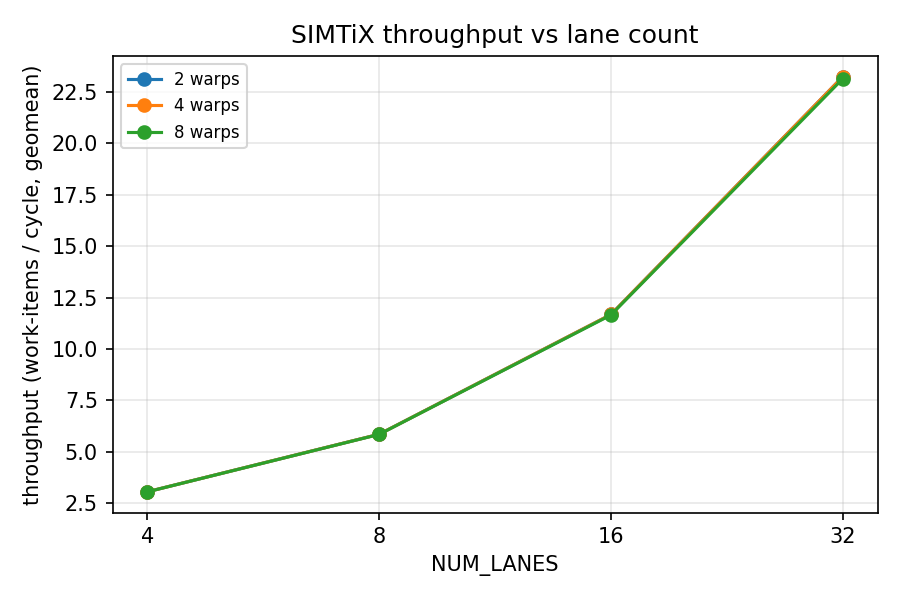
\includegraphics[width=\columnwidth]{dse_throughput.png}
\caption{Throughput versus lane count for each resident-warp count. Throughput
scales near-linearly with lanes; the warp-count curves coincide because the
single-cycle memory model offers little latency to hide.}
\label{fig:dse}
\end{figure}

%==============================================================================
\section{Floating-Point Extension}\label{sec:fp}
%==============================================================================
The base engine is integer-only. We extend it with floating point in both
single (FP32) and half (FP16) precision, keeping the same SIMT structure: the
extension is a per-lane execute unit and a second per-lane register file, not a
new pipeline.

\subsection{Per-lane FP unit and register file}
Each lane gains a compact, single-cycle floating-point unit beside its integer
ALU, and a second per-lane register file holds the 32 floating-point registers
in distributed RAM, addressed by \{warp, register\} exactly like the integer VRF.
The two files have independent write ports, so an FP compute result and an
integer load can retire in the same cycle; only same-file collisions defer.
The unit implements add, subtract, multiply, sign-injection, min/max, the
ordered compares, integer$\leftrightarrow$float conversion, the
FP32$\leftrightarrow$FP16 format conversions, the integer/FP bit-moves, and
classify, in both precisions. Rounding is round-to-nearest-even; float-to-integer
truncates; subnormals are flushed to zero in both formats, a deliberate
throughput-oriented choice that keeps each lane small. Fused multiply-add and
division/square-root are deferred to a shared per-warp special-function unit
(Section~\ref{sec:future}).

\subsection{Half precision via NaN-boxed widen--compute--narrow}
Half precision is not a second arithmetic datapath. A 16-bit half lives in a
32-bit register NaN-boxed (the upper 16 bits all ones); a mis-boxed value reads
as a canonical NaN, per the RISC-V convention. For an FP16 operation the unit
checks the box, widens the operand exactly to FP32, runs the single-precision
adder/multiplier, and rounds the FP32 result back to FP16. This is correct, not
approximate: because the FP32 intermediate carries a 24-bit significand and
$24 \ge 2\cdot 11 + 2$, rounding the exact result first to FP32 and then to FP16
gives the same value as rounding directly to FP16~\cite{figueroa}, so FP16
add/sub/mul and integer$\leftrightarrow$FP16 conversion are correctly
single-rounded. Sign-injection, min/max, comparison, classification, and the
bit-moves are done natively at 16 bits so NaN payloads and the signalling/quiet
distinction survive. Half precision thus reuses the verified single-precision
logic almost entirely, adding only the widen, narrow, and box steps.

\subsection{Verification}
The unit is verified standalone against a DPI-C IEEE-754 reference: FP32 against
the host's hardware \texttt{float}, and FP16 against a \texttt{double}-based
reference that is independent of, and was cross-checked against, the host
\texttt{\_Float16} type. Over random normal-range vectors plus directed
infinity/NaN/zero/flush-to-zero/overflow corners, a mis-NaN-boxed-operand case,
and all conversions, $76{,}048$ results match bit-for-bit with zero mismatches
(Table~\ref{tab:fpverif}). Two end-to-end kernels---$C_i=A_i+B_i$ and
$C_i=A_iB_i+B_i$---then run through the complete warp pool in each precision and
match the reference bit-exact up to 1024 threads.

\begin{table}[t]
\caption{Floating-point operation coverage. Every operation is implemented and
checked in both FP32 and FP16; all checks are bit-exact against an IEEE-754
reference.}
\label{tab:fpverif}
\centering
\footnotesize
\begin{tabular}{ll}
\toprule
Category & Operations (each in FP32 \emph{and} FP16)\\
\midrule
Arithmetic     & \texttt{fadd}, \texttt{fsub}, \texttt{fmul}\\
Sign / select  & \texttt{fsgnj\{,n,x\}}, \texttt{fmin}, \texttt{fmax}\\
Compare        & \texttt{feq}, \texttt{flt}, \texttt{fle}\\
Convert        & float$\leftrightarrow$int (signed/unsigned), FP32$\leftrightarrow$FP16\\
Move / classify& \texttt{fmv.x.\_}, \texttt{fmv.\_.x}, \texttt{fclass}\\
\midrule
\multicolumn{2}{l}{Bit-exact checks vs IEEE reference: \textbf{76{,}048} (0 mismatches)}\\
\bottomrule
\end{tabular}
\end{table}

\subsection{Floating-point throughput}
Because the FP unit is single-cycle, floating-point work flows through the SIMT
pipeline exactly like integer work. Figure~\ref{fig:fpthr} plots throughput
against problem size for streaming add and multiply-add kernels in both
precisions. The curves show the same latency-hiding ramp as the integer suite
and saturate near 7 work-items per cycle at full (100\%) lane utilization, with
coalesced traffic of three line transactions per warp. Critically, the FP16
curves lie exactly on the FP32 curves, and the cycle counts are identical
(Figure~\ref{fig:fpcost}): half precision shares the single-cycle datapath, so it
costs no extra time. Half precision therefore delivers reduced storage and
bandwidth and ISA-level FP16 support at \emph{no} throughput penalty; its area
benefit is quantified in the forthcoming per-configuration PPA sweep
(Section~\ref{sec:future}).

\begin{figure}[t]
\centering
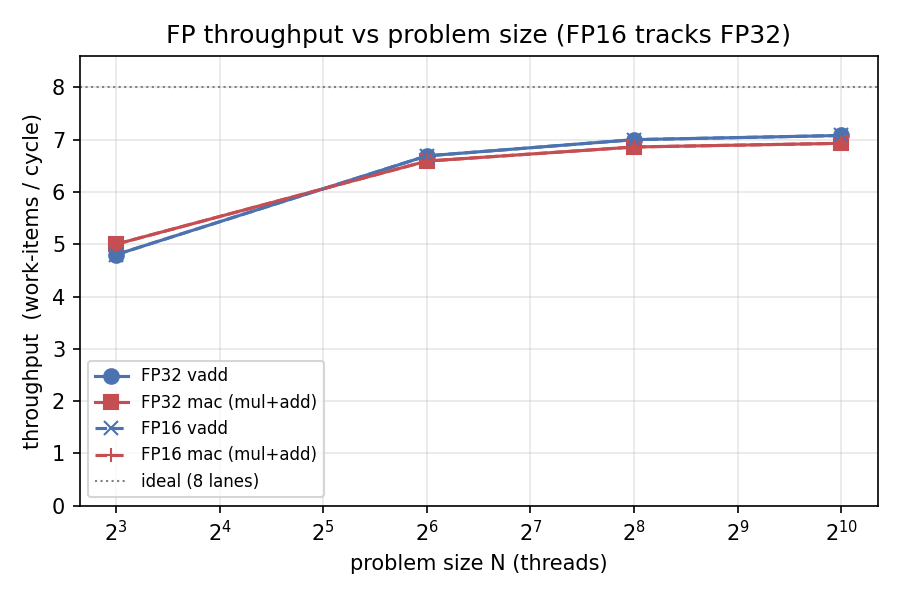
\includegraphics[width=\columnwidth]{fp_throughput.png}
\caption{Floating-point throughput versus problem size for streaming add and
multiply-add kernels. The ramp is the same latency-hiding behavior as the
integer suite; the FP16 curves coincide with the FP32 ones because both use the
single-cycle datapath.}
\label{fig:fpthr}
\end{figure}

\begin{figure}[t]
\centering
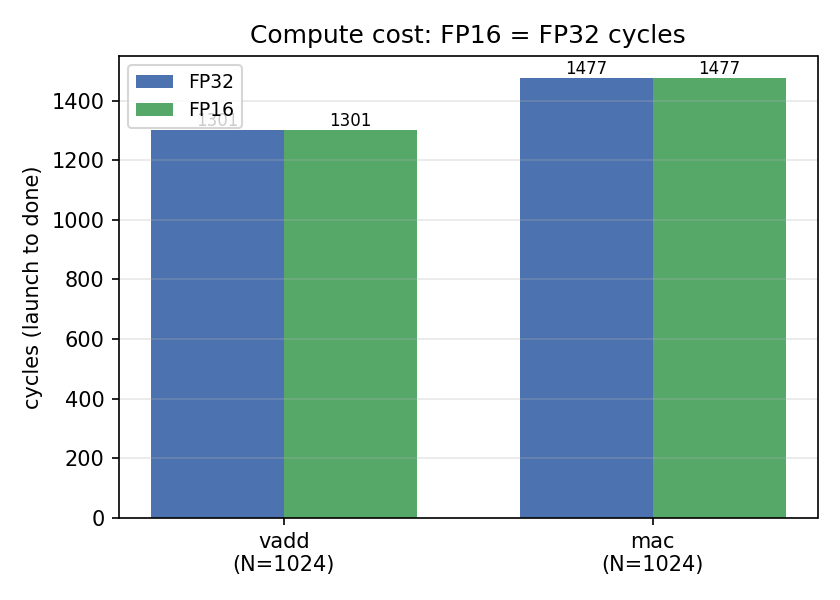
\includegraphics[width=0.74\columnwidth]{fp_cost.png}
\caption{Cycles to completion at $N{=}1024$: FP16 equals FP32 for both kernels,
confirming half precision adds no compute-time cost on the single-cycle FP unit.}
\label{fig:fpcost}
\end{figure}

%==============================================================================
\section{Related Work}\label{sec:related}
%==============================================================================
Open RISC-V GPGPU cores include Vortex~\cite{vortex}, a full OpenCL-capable
multi-core design, and Ventus~\cite{ventus}, a PTX/Vortex-style GPGPU; both
target performance and scale and are correspondingly large. Simty~\cite{simty}
demonstrates generalized SIMT execution of the RISC-V ISA, and
Nyuzi~\cite{nyuzi} is a synthesizable vector GPGPU for graphics research.
Relative to these, SIMTiX is deliberately small and readable, and its
contribution is not raw performance but a complete, reproducible RTL-to-bitstream
flow paired with a measured, mechanism-isolating evaluation and an energy-aware
divergence study. Control-divergence handling via reconvergence stacks and
dynamic warp formation is long studied~\cite{fung,tesla}; we use the standard
stack mechanism and instead \emph{measure} its energy implication through
mask-driven lane clock-gating.

%==============================================================================
\section{Discussion and Future Work}\label{sec:future}
%==============================================================================
The evaluation points to concrete next steps. The single shared data port caps
throughput below the lane-count ideal; multiple memory ports or banked access
would raise the saturation point. The \texttt{reduce} result motivates a
dedicated cross-lane reduction primitive. The lane clock-gating model is
analytic from counters; a gate-level power simulation would confirm the realized
savings. The floating-point unit (Section~\ref{sec:fp}) currently covers
add/multiply/convert in both precisions; a shared per-warp special-function unit
for division, square root, and fused multiply-add---with the multi-cycle
issue/writeback scoreboard those require---is the next extension, after which the
FP-enabled design enters the PPA sweep. The throughput design-space sweep
(Section~\ref{sec:dse}) establishes how performance scales with lanes and warps;
the complementary piece in progress is a per-configuration FPGA and ASIC PPA
sweep to complete the area/frequency/throughput Pareto. Finally, an open-source ASIC path through the
SkyWater~130\,nm PDK~\cite{sky130} using OpenLane~\cite{openlane} would turn the
FPGA PPA numbers into silicon-relevant area, frequency, and power.

%==============================================================================
\section{Conclusion}
%==============================================================================
SIMTiX shows that the full SIMT mechanism set---warp scheduling and latency
hiding, memory coalescing, a reconvergence stack, and a scratchpad---fits in a
compact, fully-open RISC-V accelerator that runs end-to-end through a real
implementation flow. A distributed-RAM register file is the key to making it
small and fast on FPGA. Across a verified six-kernel suite, SIMTiX delivers
$7$--$10\times$ measured speedup where the SIMT model fits, degrades gracefully
under divergence, and---reported honestly---loses on a serial reduction, while
its mask-driven clock-gating saves up to 22.5\% of lane-datapath dynamic energy
on divergent code. A per-lane floating-point unit adds FP32 and FP16 arithmetic,
with half precision obtained almost for free from the single-precision path by
NaN-boxed widen--compute--narrow and verified bit-exact against an IEEE
reference, sustaining the engine's full throughput at no extra cycle cost. The design and its evaluation infrastructure are public, so
the results are reproducible and the platform is reusable for teaching and
research.

%==============================================================================
\begin{thebibliography}{99}
\bibitem{vortex} B.~Tine, K.~P.~Yalamarthy, F.~Elsabbagh, and H.~Kim,
``Vortex: Extending the RISC-V ISA for GPGPU and 3D-Graphics,'' in
\emph{Proc. IEEE/ACM MICRO}, 2021.
\bibitem{ventus} F.~Zhang \emph{et al.}, ``Ventus: a RISC-V based GPGPU,''
open-source project, 2022.
\bibitem{simty} S.~Collange, ``Simty: Generalized SIMT execution on RISC-V,''
in \emph{Workshop on Computer Architecture Research with RISC-V (CARRV)}, 2017.
\bibitem{nyuzi} J.~Bush, P.~Dexter, T.~N.~Miller, and A.~Carpenter,
``Nyami: a synthesizable GPU architectural model for general-purpose and
graphics-specific workloads,'' in \emph{Proc. IEEE ISPASS}, 2015.
\bibitem{fung} W.~W.~L.~Fung, I.~Sham, G.~Yuan, and T.~M.~Aamodt,
``Dynamic Warp Formation and Scheduling for Efficient GPU Control Flow,'' in
\emph{Proc. IEEE/ACM MICRO}, 2007.
\bibitem{tesla} E.~Lindholm, J.~Nickolls, S.~Oberman, and J.~Montrym,
``NVIDIA Tesla: A Unified Graphics and Computing Architecture,''
\emph{IEEE Micro}, vol.~28, no.~2, 2008.
\bibitem{sky130} SkyWater Technology and Google, ``SkyWater Open Source PDK
(sky130),'' \url{https://github.com/google/skywater-pdk}.
\bibitem{openlane} A.~Ghazy and M.~Shalan, ``OpenLane: The Open-Source Digital
ASIC Implementation Flow,'' in \emph{Workshop on Open-Source EDA Technology
(WOSET)}, 2020.
\bibitem{riscv} A.~Waterman and K.~Asanovi\'c, ``The RISC-V Instruction Set
Manual, Volume I: Unprivileged ISA,'' RISC-V International.
\bibitem{figueroa} S.~A.~Figueroa, ``When is double rounding innocuous?,''
\emph{ACM SIGNUM Newsletter}, vol.~30, no.~3, pp.~21--26, 1995.
\end{thebibliography}

\end{document}
